\documentclass[11pt]{article}

\usepackage[T1]{fontenc}
\usepackage{amsmath,amssymb}
\usepackage{booktabs}
\usepackage{geometry}
\usepackage{graphicx}
\usepackage{hyperref}
\usepackage{microtype}
\usepackage{xcolor}

\geometry{margin=1in}
\graphicspath{{./}}
\hypersetup{colorlinks=true,linkcolor=blue!55!black,urlcolor=blue!55!black}

\newcommand{\fro}{\mathrm{F}}
\newcommand{\RR}{\mathbb{R}}
\newcommand{\code}[1]{\texttt{#1}}

\title{QHO1D Spatial Truncation\\
\large Finite-box and finite-difference technical report}
\author{Project Koios}
\date{\today}

\begin{document}
\maketitle

\begin{center}
\fbox{\begin{minipage}{0.92\linewidth}
\textbf{Status.} This is a mutable technical report for
\code{calculations/qho1d}. It is not retained evidence, a publication manuscript,
a continuum-convergence proof, or a physical uncertainty statement. The plotted
arrays are binary64 development outputs. Exact Lean results are cited separately and
do not certify the runtime arrays in this experiment.
\end{minipage}}
\end{center}

\begin{abstract}
This report studies spatial truncation: how a one-dimensional quantum harmonic
oscillator on the real line changes when represented on a finite Dirichlet box and
grid, then compared with a retained number-state reference.  The
experiment compares a centered second-order finite-difference Hamiltonian with the
direct diagonal number-state Hamiltonian after sampled Hermite states have been
Gram-orthonormalized and used as a common-coordinate injection.  It records
Frobenius, diagonal, off-diagonal, Gram, isometry, refinement, eigenvalue, eigenstate,
and residual diagnostics.  The development sweep demonstrates the expected
second-order spatial trend once the finite box is sufficiently large, while a smaller
box exhibits a distinct boundary-dominated regime.  Formal results establish the
exact Hermite--Gaussian pointwise eigenfunction identity, finite ladder boundary
defect, compression leakage identity, and conditional common-coordinate algebra.
They deliberately do not establish the remaining finite-box, discretization, or
floating-point error bounds.
\end{abstract}

\section{Question and scope}

The computational question is not whether the harmonic oscillator is analytically
solvable.  It is how several finite representations differ when they are compared in
one explicitly constructed coordinate space.  For box half-width $b$, realized grid
spacing $h$, and retained Python dimension $K$, the experiment constructs
\begin{equation}
  D_{b,h,K}=J^{\mathsf T}H_{b,h}J-H_K.
  \label{eq:difference}
\end{equation}
Here $H_{b,h}$ is the finite Dirichlet-grid Hamiltonian, $H_K$ is the direct diagonal
reference with entries $n+\tfrac12$ for $n=0,\ldots,K-1$, and $J$ maps retained
number-state coordinates into the interior grid.

The experiment is nondimensional with
$\hbar=m=\omega=\ell=1$.  It does not claim that a finite grid is the continuum
operator, that the selected sweep proves convergence, or that the discrepancy is a
single uncertainty estimate.  Its purpose is to expose separately measurable error
channels and to provide reusable diagnostics for later certified bounds.

\section{Representations and comparison map}

Let $x_i$ denote the ordered interior coordinates of a uniform grid on $[-b,b]$ with
homogeneous Dirichlet endpoints.  The spatial matrix uses the centered stencil
\begin{equation}
  (\Delta_h f)_i=\frac{f_{i-1}-2f_i+f_{i+1}}{h^2},
  \qquad
  H_{b,h}=-\frac12\Delta_h+\frac12\operatorname{diag}(x_i^2).
\end{equation}
The real-line spectral problem and its Hermite-state solution are standard
\cite{shankar1994,teschl2014}. The exact real-line number-state samples are
\begin{equation}
  \psi_n(x)=\frac{H_n(x)e^{-x^2/2}}{\pi^{1/4}\sqrt{2^n n!}},
  \qquad E_n=n+\frac12.
\end{equation}
The implementation evaluates the normalized states through their stable three-term
recurrence.  With $S_{in}=\sqrt{h}\,\psi_n(x_i)$, it constructs
\begin{equation}
  G=S^{\mathsf T}S,\qquad R=G^{-1/2},\qquad J=SR.
  \label{eq:gram-map}
\end{equation}
The inverse square root is computed from a binary64 symmetric eigendecomposition using
standard finite matrix methods \cite{golubVanLoan2013}. It is therefore checked
numerically; it is not the exact inverse square root assumed by the corresponding Lean
isometry theorem.

The direct diagonal definition of $H_K$ is intentional.  Constructing the Hamiltonian
from products of already-truncated ladder matrices introduces a highest-state boundary
defect even before spatial discretization is considered.

\section{Formal crosswalk}

The proof sidecar uses Lean~4 and mathlib
\cite{demouraUllrich2021,mathlib2020} in the \code{projectkoios-formal} repository at
local commit
\begin{center}
\small\code{002e1a2b4167acf9fe467a4f3da733c23dfd28e1}.
\end{center}
The following results are used as mathematical boundaries rather than runtime
certificates.

\begin{table}[ht]
\centering
\small
\begin{tabular}{@{}p{0.25\linewidth}p{0.65\linewidth}@{}}
\toprule
Formal identifier & Relevance to this experiment \\
\midrule
\code{QHO-HERMITE-THM-001} & The constructed physicists' Hermite polynomials satisfy
the exact differential equation. \\
\code{QHO-HERMITE-THM-002} & The unnormalized Hermite--Gaussian satisfies the
pointwise dimensionless oscillator eigenfunction identity with eigenvalue
$n+\tfrac12$.  This is not an $L^2$ completeness theorem. \\
\code{QHO-LADDER-THM-001} & A retained ladder commutator equals
$I-(K_{\!F}+1)|K_{\!F}\rangle\langle K_{\!F}|$ in formal dimension $K_{\!F}+1$. \\
\code{QHO-TRUNCATION-THM-001} & Compression fails to preserve products by the exact
omitted-space leakage term $J^{\mathsf T}A(I-JJ^{\mathsf T})BJ$. \\
\code{QHO-TRUNCATION-THM-002} & Reconstructing the oscillator Hamiltonian from
truncated ladder products subtracts an explicit highest-state projector term. \\
\code{QHO-COMPARISON-THM-001} & If
$R^{\mathsf T}(S^{\mathsf T}S)R=I$ exactly, then $J=SR$ is exactly isometric. \\
\code{QHO-COMPARISON-THM-002} & The squared finite-matrix Frobenius magnitude splits
exactly into diagonal and off-diagonal contributions. \\
\bottomrule
\end{tabular}
\caption{Exact proof results and their deliberately bounded applicability.}
\label{tab:formal-crosswalk}
\end{table}

The formal cutoff $K_{\!F}$ labels the highest retained state and has dimension
$K_{\!F}+1$.  The Python field \code{retained\_dimension} is the dimension $K$ and
contains states $0$ through $K-1$.  Thus $K_{\!F}=K-1$ for every nonempty Python case.
The audited Lean proofs contain no \code{sorry}; their reported transitive foundations
are limited to the repository's disclosed standard classical axioms.  No theorem binds
the exact matrices directly to the JSON bytes produced here.

\section{Development protocol}

The declared Cartesian sweep is
\begin{equation}
 b\in\{4,6,8\},\qquad
 h_{\mathrm{requested}}\in\{0.2,0.1,0.05\},\qquad
 K\in\{2,4,6\}.
\end{equation}
This produces 27 deterministically ordered cases.  Each case retains the realized
spacing, interior-point count, comparison-map content hash, Gram matrix, inverse Gram
square root, pulled-back Hamiltonian, direct reference, signed difference, and scalar
diagnostics.  Cross-grid records compare adjacent spatial resolutions while holding
$b$ and $K$ fixed.

The implementation is library-owned by
\code{ksdft2effmass.model\_systems.qho1d}.  The experiment directory owns only the
input, development entry points, this report, and replaceable outputs.  The finite
difference, ladder, and typed-quantity mechanisms reuse existing
\code{ksdft2effmass.operators} components.

\section{Eigenstates and finite-grid distortion}

Figure~\ref{fig:eigenstates} compares the first four real-line Hermite states against
the sign-aligned eigenvectors of the finite Dirichlet-grid Hamiltonian for
$b=8$, $h=0.05$, and $K=6$.  A Euclidean-normalized grid eigenvector $v_n$ is displayed
as $v_n/\sqrt{h}$ so that $h\sum_i|v_{n,i}/\sqrt{h}|^2=1$.  The sign is chosen only for
visual comparison and carries no physical content.

\begin{figure}[ht]
\centering
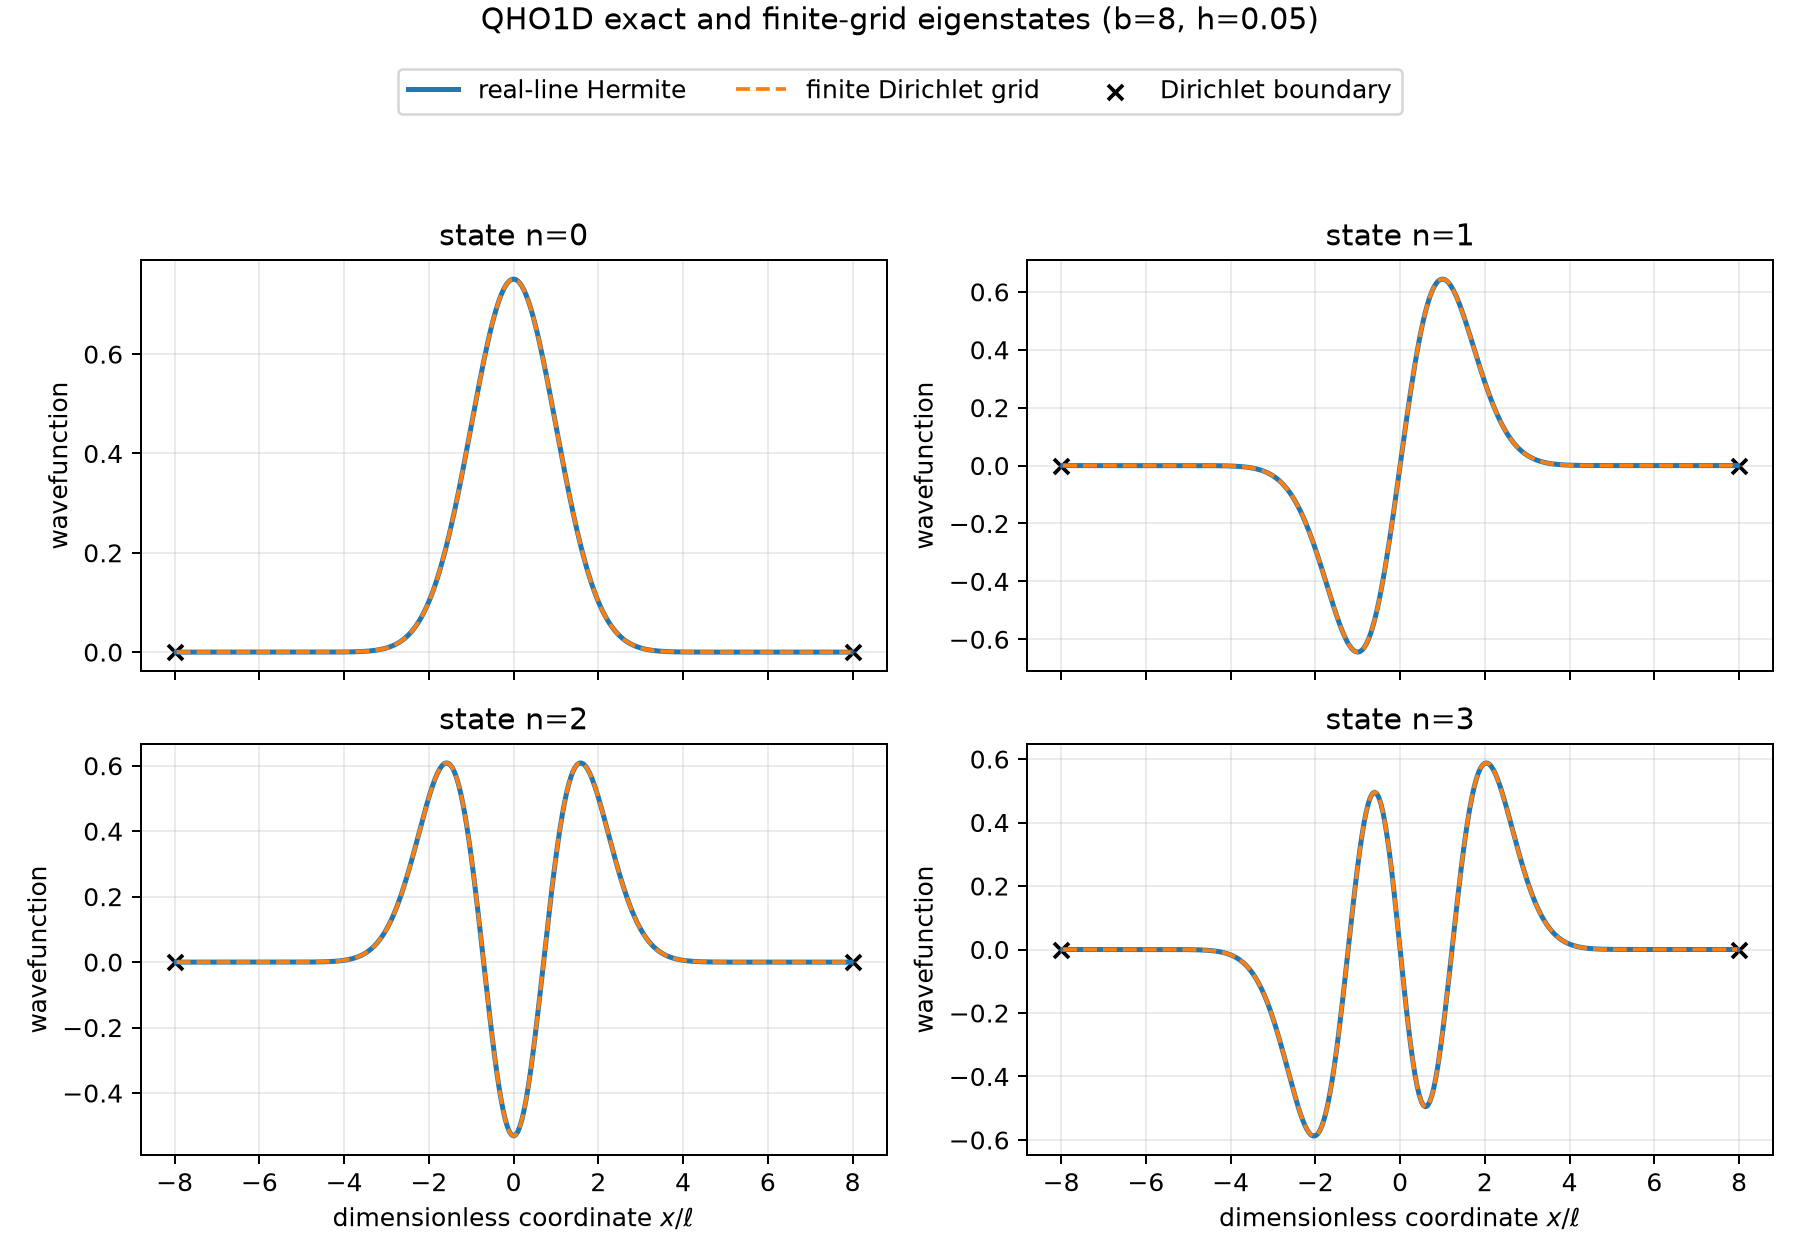
\includegraphics[width=\linewidth]{qho1d-eigenstates.png}
\caption{Real-line Hermite states and finite-grid eigenstates for the selected fine
case.  The agreement at plot scale does not replace the distortion diagnostics.}
\label{fig:eigenstates}
\end{figure}

Figure~\ref{fig:state-distortion} exposes the difference hidden by the overlay.  For
states $n=0,1,2,3$, the grid-weighted state-difference norms are approximately
$1.15\times10^{-4}$, $3.27\times10^{-4}$, $6.53\times10^{-4}$, and
$1.11\times10^{-3}$.  The finite-grid energy errors for $n=0,\ldots,5$ are
\begin{equation}
 (-7.81\!\times\!10^{-5},-3.91\!\times\!10^{-4},-1.02\!\times\!10^{-3},
 -1.95\!\times\!10^{-3},-3.21\!\times\!10^{-3},-4.77\!\times\!10^{-3}).
\end{equation}
These are development observations for one selected grid, not spectral enclosures.

\begin{figure}[ht]
\centering
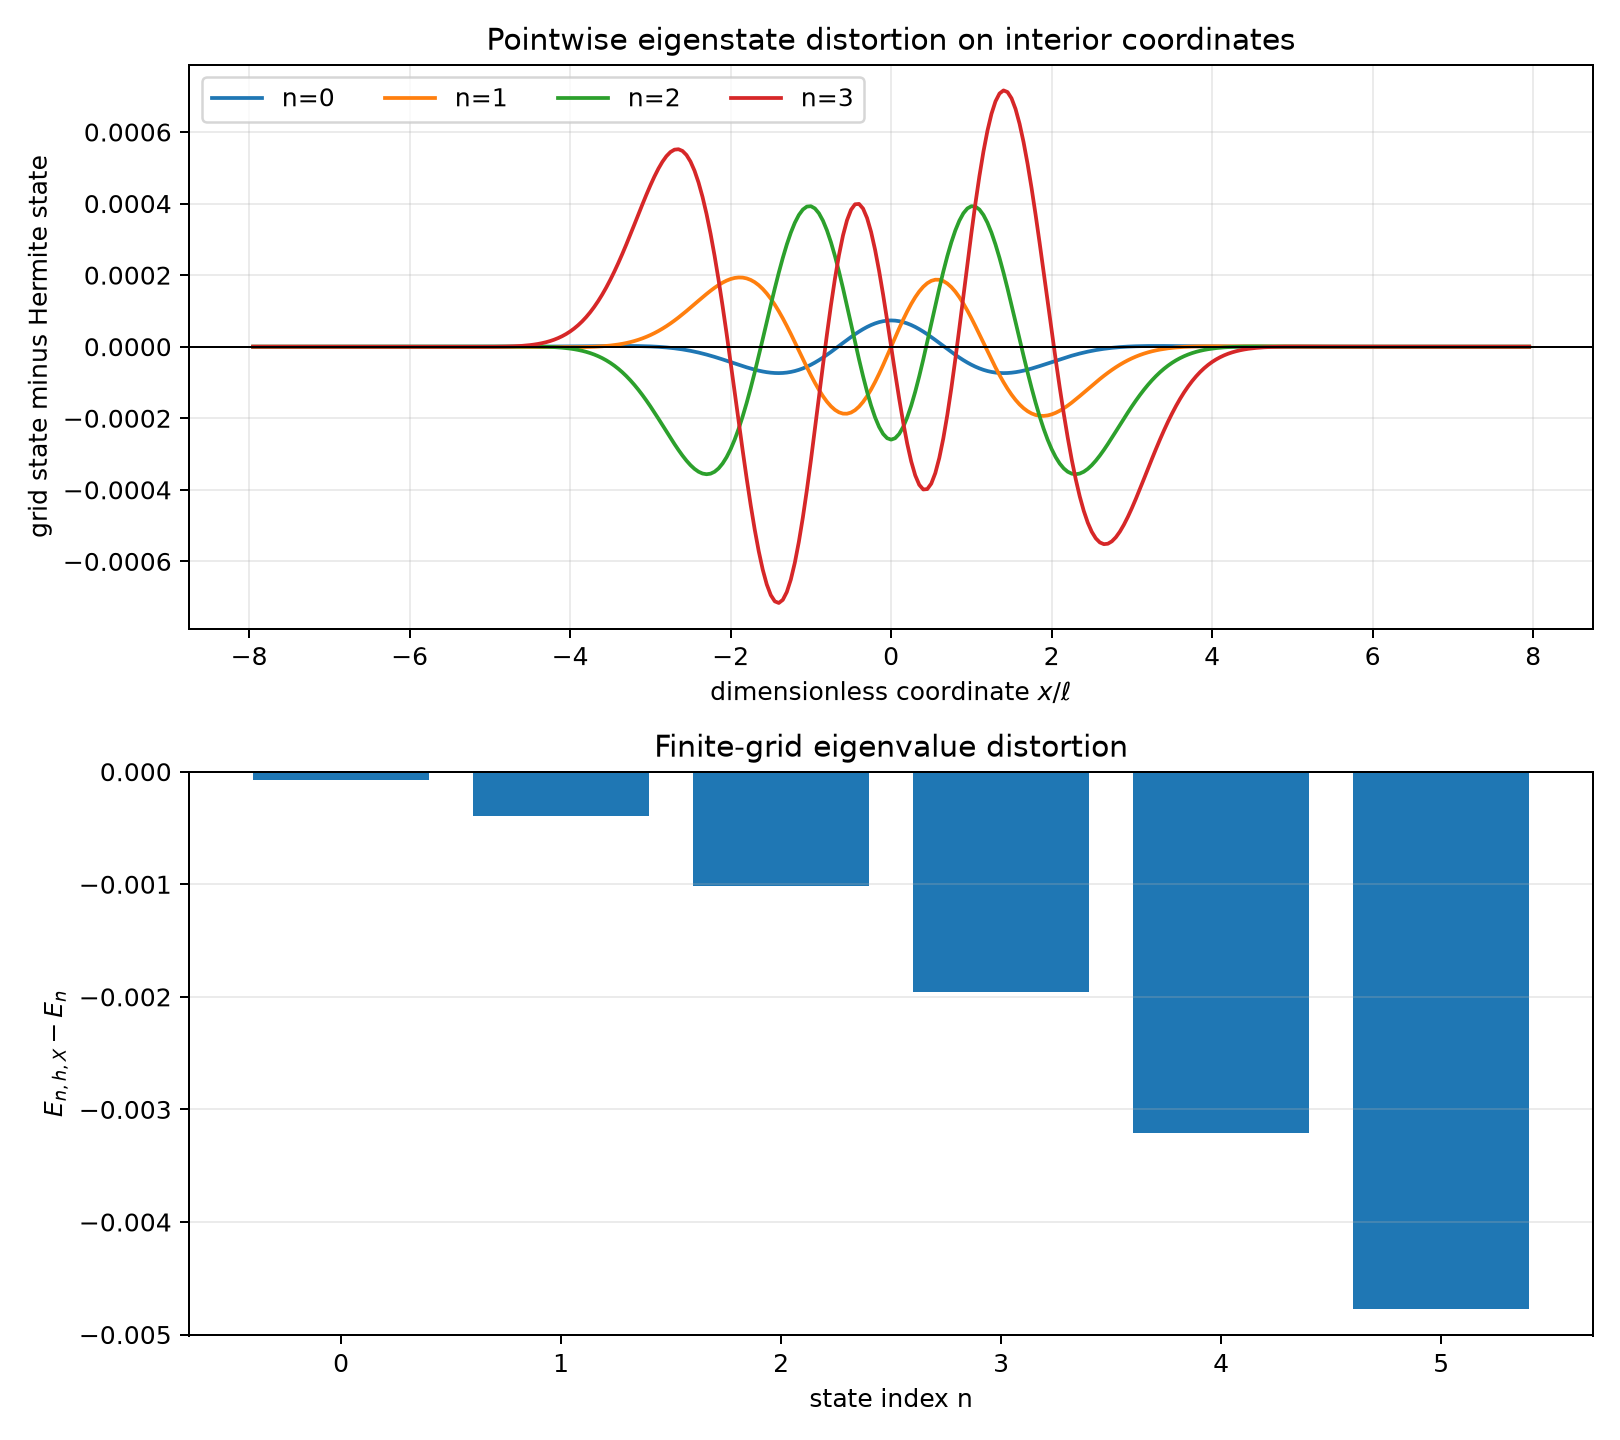
\includegraphics[width=0.94\linewidth]{qho1d-eigenstate-distortion.png}
\caption{Pointwise state distortion and finite-grid eigenvalue distortion for
$b=8$, $h=0.05$, and the first six eigenvalues.}
\label{fig:state-distortion}
\end{figure}

\section{Reusable diagnostics}

For each case the result records
\begin{align}
 \delta_{\mathrm{abs}} &= \|D_{b,h,K}\|_{\fro}, &
 \delta_{\mathrm{rel}} &=
 \frac{\|D_{b,h,K}\|_{\fro}}{\|H_K\|_{\fro}},\\
 \delta_G &= \|G-I\|_{\fro}, &
 \delta_J &= \|J^{\mathsf T}J-I\|_{\fro}.
\end{align}
It also records $\|\operatorname{diag}D\|_{\fro}$ and
$\|D-\operatorname{diag}D\|_{\fro}$.  These channels distinguish normalization and
common-coordinate effects from diagonal energy shifts and representation-induced
couplings.

A further reusable a-posteriori diagnostic is
\begin{equation}
  \rho_{b,h,K}=\|H_{b,h}J-JH_K\|_{\fro}.
  \label{eq:residual}
\end{equation}
For an exact isometry $J^{\mathsf T}J=I$,
\begin{equation}
  J^{\mathsf T}H_{b,h}J-H_K
  =J^{\mathsf T}(H_{b,h}J-JH_K),
\end{equation}
so $\delta_{\mathrm{abs}}\leq\rho_{b,h,K}$ in the Euclidean operator/Frobenius
bound.  The plot reports the binary64 evaluation of both quantities.  It is not an
interval-certified inequality.

\begin{figure}[ht]
\centering
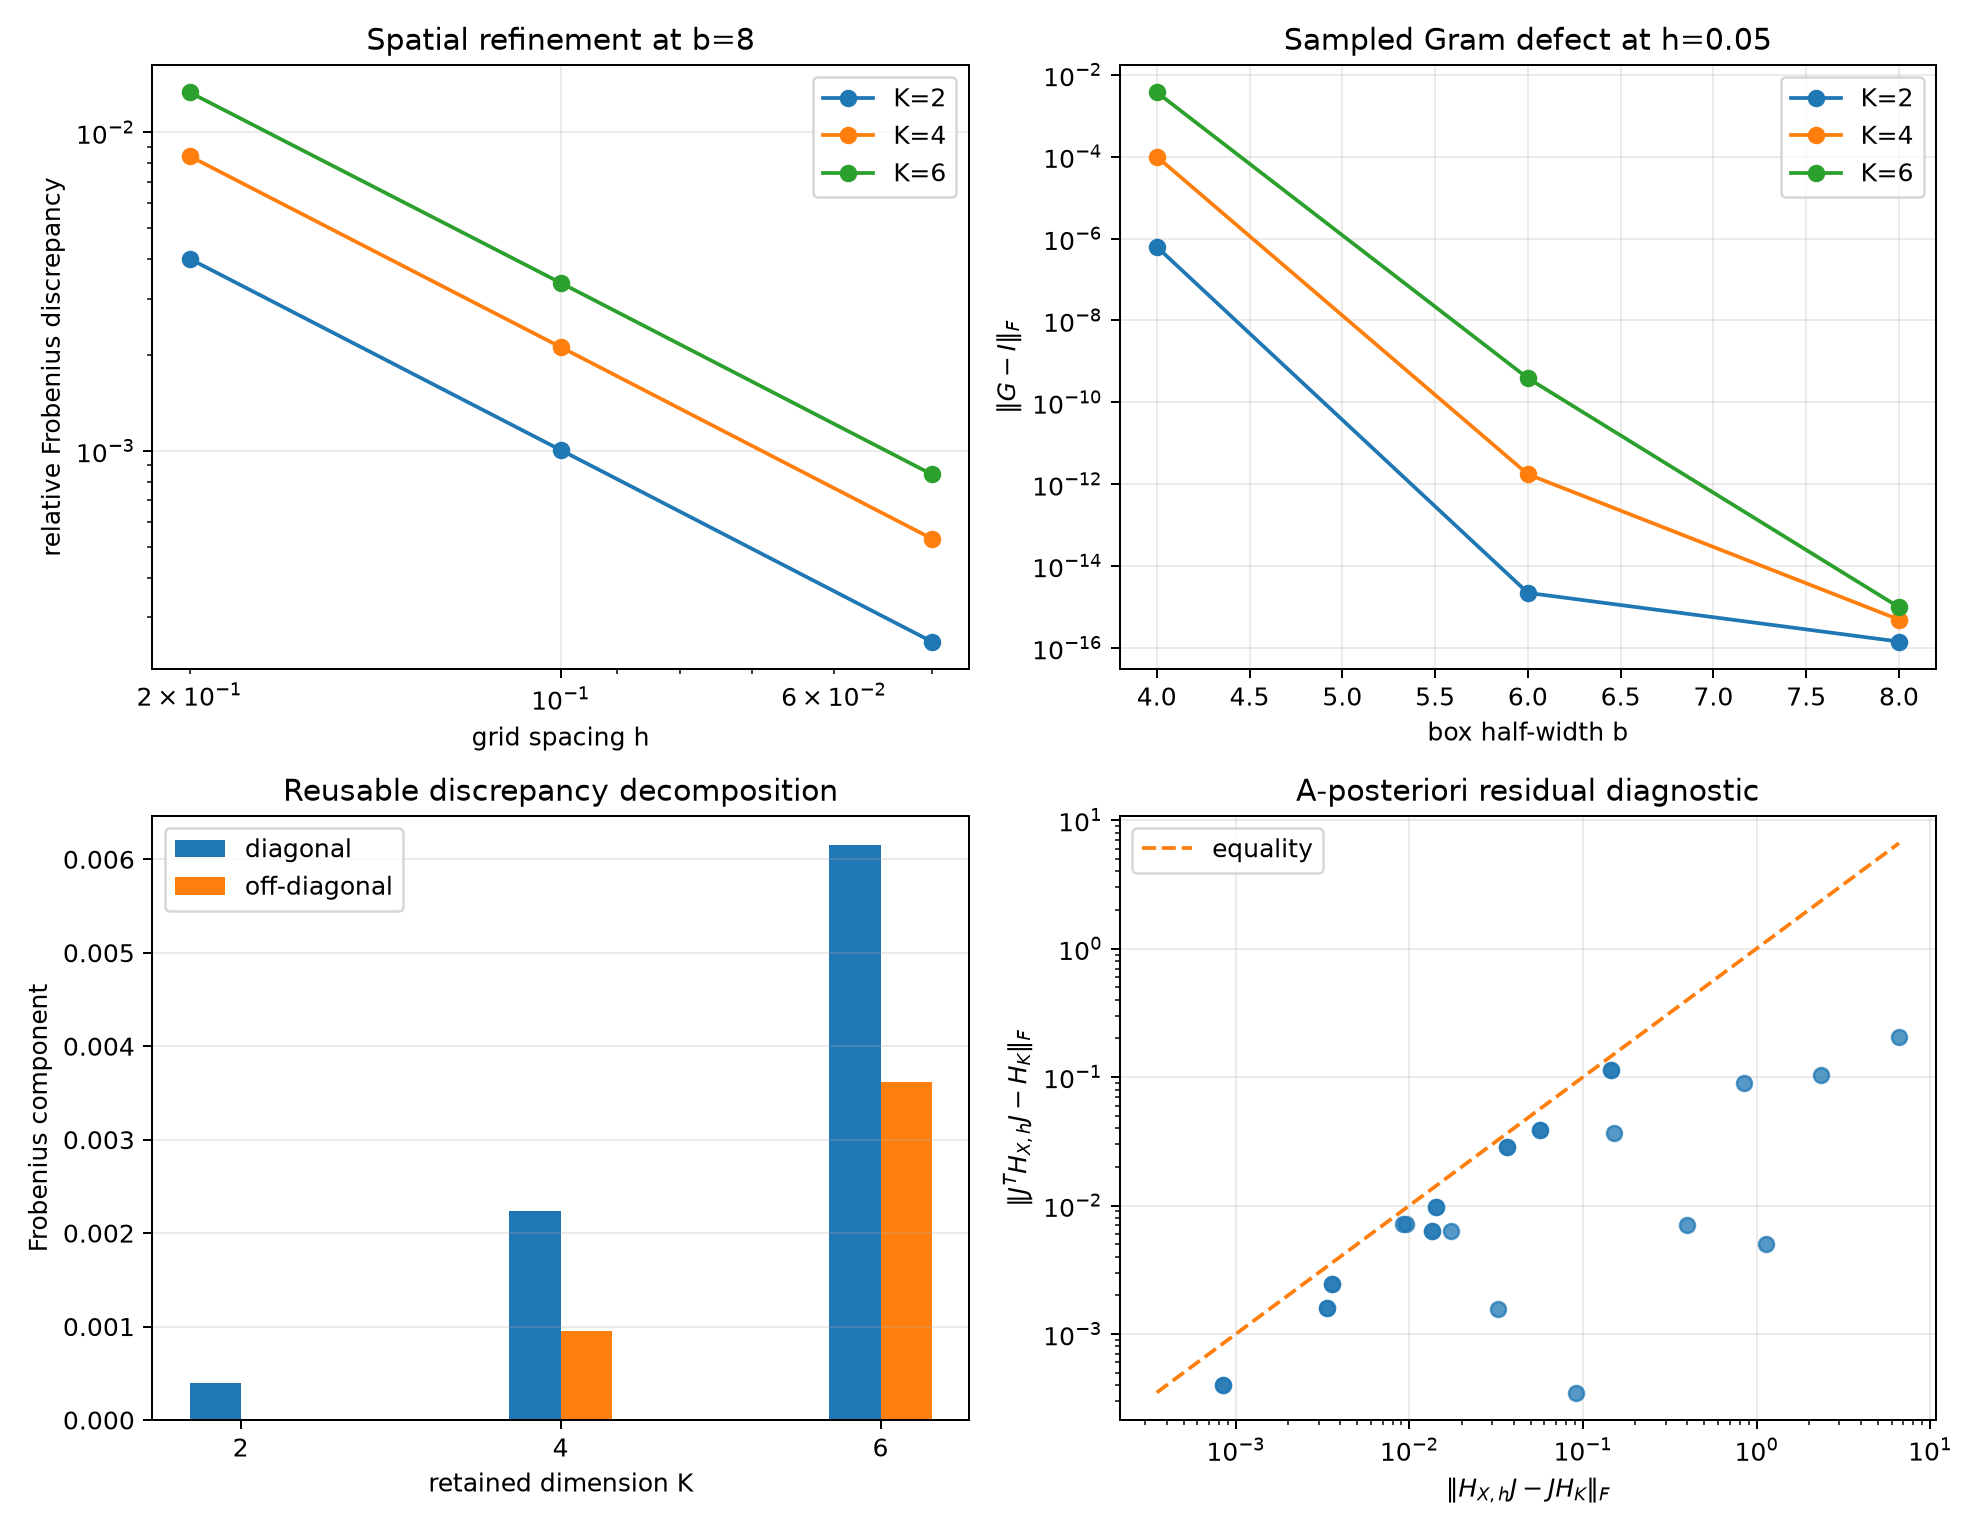
\includegraphics[width=\linewidth]{qho1d-diagnostics.png}
\caption{Spatial refinement, sampled Gram defect, diagonal/off-diagonal decomposition,
and residual diagnostic.  Every panel reports mutable binary64 development data.}
\label{fig:diagnostics}
\end{figure}

\section{Observed regimes}

Table~\ref{tab:k6-results} shows the relative discrepancy for the largest retained
space.  At $b=6$ and $b=8$, halving $h$ reduces the discrepancy by factors close to
four, consistent with the expected centered-difference order over this limited sweep.
This is an observed trend, not a proof or fitted asymptotic bound.  Results for
$b=6$ and $b=8$ are nearly identical at the displayed scale, indicating that the
real-line tails are below the leading discretization effect for these cases.

At $b=4$, refinement does not improve the combined discrepancy and ultimately makes
it larger.  The sampled Gram defect is also much larger.  This is useful rather than
pathological: it demonstrates that grid refinement cannot be interpreted without a
separate finite-box channel.  A finer stencil resolves the fixed, boundary-incompatible
box problem more accurately; it does not turn that problem into the real-line
oscillator.

\begin{table}[ht]
\centering
\begin{tabular}{@{}cccc@{}}
\toprule
$b$ & $h$ & $K$ & $\delta_{\mathrm{rel}}$ \\
\midrule
4 & 0.20 & 6 & $1.0570\times10^{-2}$ \\
4 & 0.10 & 6 & $1.2283\times10^{-2}$ \\
4 & 0.05 & 6 & $2.4372\times10^{-2}$ \\
6 & 0.20 & 6 & $1.3370\times10^{-2}$ \\
6 & 0.10 & 6 & $3.3708\times10^{-3}$ \\
6 & 0.05 & 6 & $8.4448\times10^{-4}$ \\
8 & 0.20 & 6 & $1.3370\times10^{-2}$ \\
8 & 0.10 & 6 & $3.3708\times10^{-3}$ \\
8 & 0.05 & 6 & $8.4448\times10^{-4}$ \\
\bottomrule
\end{tabular}
\caption{Relative common-coordinate Frobenius discrepancy for $K=6$.}
\label{tab:k6-results}
\end{table}

For the selected $(b,h,K)=(8,0.05,6)$ case, the absolute discrepancy is
$7.1407\times10^{-3}$; its diagonal and off-diagonal components are
$6.1581\times10^{-3}$ and $3.6150\times10^{-3}$, respectively.  Their squared values,
not their values, add to the squared total as established by the exact finite-matrix
decomposition.  The Gram defect is $9.93\times10^{-16}$ and the measured injection
isometry error is $3.22\times10^{-15}$, both at binary64 scale for this case.

\section{Error-channel ledger}

The observed discrepancy must not be collapsed into one unnamed error.  The current
ledger is:
\begin{enumerate}
\item \textbf{Exact finite ladder truncation.} Truncated ladder products have an
explicit top-state boundary defect.  The Python comparison avoids this channel by
using the direct diagonal reference.
\item \textbf{Finite-box closure.} Real-line Hermite states do not exactly satisfy a
finite homogeneous Dirichlet boundary.  The $b=4$ observations show that this channel
can dominate refinement.
\item \textbf{Interior discretization.} The centered stencil has the standard local
second-order consistency mechanism \cite{strikwerda2004}, but this report does not
supply a governed global
constant or regularity-to-spectrum theorem.
\item \textbf{Sampled-state and Gram correction.} Finite quadrature changes the Gram
matrix, and numerical inverse-square-root normalization changes the sampled columns.
\item \textbf{Projection and pullback.} $J^{\mathsf T}H_{b,h}J$ measures the operator
in one retained coordinate space; it is not the full grid spectrum.
\item \textbf{Eigensolver and floating point.} Every runtime matrix, eigendecomposition,
norm, and serialized decimal is binary64 and has no interval certificate here.
\end{enumerate}

\section{Reproduction and provenance}

From the repository's \code{python/} directory, the mutable development workflow is
\begin{verbatim}
uv run python ../calculations/qho1d/dev_analysis.py
uv run python ../calculations/qho1d/dev_verification.py
uv run python ../calculations/qho1d/dev_plots.py
\end{verbatim}
The fixed result path is
\code{calculations/qho1d/analysis/development/qho1d-result.json}.  The current generated
result has SHA-256
\begin{center}
\small\code{e22e83398b7f77d1ad3717e6789da30847092af5eebf5af4ebe9c7f7d57ac25d}.
\end{center}
This digest identifies only the present replaceable development bytes; it does not
promote them to retained evidence.  The JSON independently records input, runner, and
implementation-file identities and is checked by the QHO1D result verifier before the
plots are produced.

\section{Next steps}

The next useful result is a channel-separated bound, not a larger undifferentiated
sweep.  Priorities are to retain boundary-row and interior residuals separately,
serialize the full residual diagnostic, establish a governed residual-to-spectrum
statement, derive an explicit finite-box Hermite-tail estimate, and connect the
centered-difference consistency residual to a global eigenvalue/eigenstate bound.
Interval or otherwise checked floating-point certificates would be required before
promoting binary64 observations to rigorous numerical enclosures.

\bibliographystyle{plain}
\bibliography{references}

\end{document}
